\documentclass[a4paper]{article}

% Packages
\usepackage{geometry}
\geometry{left=1.5cm, right=1.5cm, top=1.5cm, bottom=2.54cm}
\usepackage{graphicx, hyperref, setspace, amsmath, amssymb, titlesec, fancyhdr, multicol, parskip, indentfirst, etoolbox, caption, cite, xcolor}
\usepackage{float}

% Title Formatting
\titleformat{\section}{\centering\large\scshape}{\thesection}{1em}{}
\titleformat{\subsection}{\normalsize\bfseries}{\thesubsection}{1em}{}
\titleformat{\subsubsection}{\normalfont\itshape}{\thesubsubsection}{1em}{}

\setstretch{1.0}
\setlength{\parskip}{6pt}
\setlength{\parindent}{0.5cm}
\titlespacing{\section}{0pt}{6pt}{6pt}
\titlespacing{\subsection}{0pt}{6pt}{6pt}
\titlespacing{\subsubsection}{0pt}{6pt}{6pt}

% Section Numbering
\renewcommand{\thesection}{\Roman{section}.}
\renewcommand{\thesubsection}{\textit{\Alph{subsection}.}}
\renewcommand{\thesubsubsection}{\textit{\arabic{subsubsection}.}}
\renewcommand{\thetable}{\Roman{table}}
\renewcommand{\thefigure}{\Roman{figure}}

% Caption Setup
\captionsetup{labelfont={small,sc}, textfont={small,sc}, labelsep=period}

% Title
\title{\textbf{Resume Screening: An AI-Driven Framework for Automated Candidate Matching}}
\date{}

% Header
\pagestyle{fancy}
\fancyhf{}
\fancyfoot[C]{\thepage} % Page number centered in the footer


\begin{document}
\maketitle
\vspace{-1.5cm}

% Authors Block
\begin{multicols}{3}
\centering
\textbf{Joel Payippara Shibu}\\
\textit{Department of Electrical and Computer Engineering}\\
\textit{Western University}\\
\textit{London, Canada}\\
\textit{jpayippa@uwo.ca}\\

\columnbreak

\textbf{Mert Osoydan}\\
\textit{Department of Computer Science}\\
\textit{Western University}\\
\textit{London, Canada}\\
\textit{mosoydan@uwo.ca}\\

\columnbreak

\textbf{Saif Ahmad}\\
\textit{Department of Electrical and Computer Engineering}\\
\textit{Western University}\\
\textit{London, Canada}\\
\textit{sahma244@uwo.ca}\\
\end{multicols}

\begin{multicols}{2}
\setlength{\columnsep}{0.5cm}


\textbf{\textit{Abstract—In this paper, we investigate the effectiveness of machine learning and natural language processing (NLP) techniques in automating the job matching process. Our system extracts and analyzes candidate qualifications and experience from resumes and aligns them with job descriptions using similarity and ranking models. Additionally, we implement a recommendation component that generates resume improvement suggestions. This work addresses common inefficiencies in traditional hiring pipelines by improving both speed and fairness in candidate screening. Evaluation demonstrates promising results, with substantial improvement in matching accuracy and reduced screening time. Future work includes adapting the system to specific industry domains for enhanced contextual relevance.}}



% =========================================================================================================================================================================================================================================================================================================================================================================================================================================================================================================================================================================================================================================================================
% =========================================================================================================================================================================================================================================================================================================================================================================================================================================================================================================================================================================================================================================================================




\section{Introduction}

Hiring remains a foundational yet labor-intensive function within organizations. As digital applications surge, recruiters face the increasingly burdensome task of reviewing hundreds—sometimes thousands—of resumes for a single role. This burden is not only quantitative but also qualitative: critical nuances in candidate experience, skill alignment, and job fit are often overlooked due to time constraints or cognitive bias. Consequently, hiring pipelines become inefficient, inconsistent, and prone to both false positives and false negatives in candidate selection.

This growing complexity has created fertile ground for artificial intelligence (AI) and machine learning (ML) solutions. In particular, natural language processing (NLP) techniques have demonstrated strong potential in parsing and extracting structured meaning from unstructured text—such as resumes and job descriptions—by transforming them into high-dimensional vector representations that capture semantic relationships. Resume-job matching, therefore, becomes a similarity problem solvable through model-driven computation.

The core objective of this project is to design a robust, intelligent system capable of identifying match quality between candidates and job postings using semantic embeddings, engineered features, and supervised learning models. Much like modern recommendation engines in retail and streaming platforms, our approach leverages similarity metrics and rank-based learning to convert human judgment into quantitative predictions.

Importantly, this system also confronts structural challenges in hiring—chiefly bias and inequity. By anonymizing sensitive information and applying fairness-aware ranking algorithms, we seek to enhance objectivity in selection processes. Moreover, by generating resume feedback, our system empowers applicants with insights traditionally reserved for career coaches or hiring professionals—helping democratize access to quality job preparation.

While prior work has applied AI to recruitment, many systems rely on keyword matching or rigid rule-based filters. Our work advances the field by incorporating sentence-transformer embeddings, efficient vector search (FAISS), and performance evaluation through metrics such as F1-score, ROC AUC, and confusion matrices.

This paper focuses not on replacing human recruiters, but on building the computational backbone for scalable, fair, and interpretable AI-assisted hiring systems. It aims to bridge the gap between human intuition and data-driven intelligence by emphasizing the design and implementation of practical, production-ready solutions.



% =========================================================================================================================================================================================================================================================================================================================================================================================================================================================================================================================================================================================================================================================================
% =========================================================================================================================================================================================================================================================================================================================================================================================================================================================================================================================================================================================================================================================================


\section{Background and Related Work}
Understanding the current research landscape is crucial to situating our system within broader advancements in AI-driven recruitment. This section examines the limitations of traditional hiring workflows, outlines recent progress in NLP-based candidate matching, and highlights the growing emphasis on fairness and explainability. We also identify gaps in the literature that this project aims to address.

\subsection{Automated Hiring and NLP in Recruitment}
Automated hiring systems emerged in response to the inefficiencies of manual resume screening, particularly in high-volume contexts. Early systems primarily relied on keyword matching and Boolean search, offering minimal semantic understanding. More recent approaches utilize NLP techniques such as Named Entity Recognition (NER), part-of-speech tagging, and syntactic parsing to extract structured features from resumes and job descriptions \cite{4}.

Advancements in pretrained language models—such as BERT \cite{2} and its sentence-level variants like Sentence-BERT \cite{3}—have enabled deeper semantic understanding. These embeddings are increasingly used in both candidate ranking and job matching systems. Tools like Workday and Eightfold.ai have already begun leveraging transformer-based architectures for resume parsing and job fit prediction.

Despite these advances, commercial Applicant Tracking Systems (ATS) largely remain limited to static rules and lack the sophistication of contextual embedding or real-time learning. Our system addresses this by incorporating semantic similarity scoring, cosine distance retrieval via FAISS \cite{6}, and ranking models for predictive classification.

\subsection{Bias and Fairness in AI Hiring}
Bias in algorithmic hiring tools has become a central concern in the literature. Studies have found that historical hiring data often reflects systemic inequalities, which, if used without corrective measures, can perpetuate discrimination across gender, race, and socioeconomic status \cite{5}.

Efforts to mitigate such risks include feature anonymization, fairness-aware loss functions, and post-hoc explainability tools. Raghavan et al. \cite{5} emphasize the importance of transparency and human-in-the-loop strategies when deploying such systems in sensitive domains like employment. In our implementation, we omit personally identifiable information and aim for equal error rates across demographic groups, setting a foundation for more robust fairness auditing in future work.

\subsection{Research Gap}
Most existing systems fall into one of two extremes: simplistic keyword filters or opaque black-box neural networks. Few offer the combination of semantic retrieval, interpretable scoring features, and modular extensibility for resume feedback generation. Additionally, there is limited open research on real-world deployment of such systems within end-to-end pipelines, particularly in resource-constrained settings.

By integrating semantic embeddings, weak supervision, and model explainability into a cohesive pipeline, this work contributes a reproducible and adaptable framework for AI-assisted hiring. It builds upon recent advances in transformer models and scalable similarity search while emphasizing human-aligned decision metrics.



% =========================================================================================================================================================================================================================================================================================================================================================================================================================================================================================================================================================================================================================================================================
% =========================================================================================================================================================================================================================================================================================================================================================================================================================================================================================================================================================================================================================================================================



\section{Methods}
Our proposed pipeline follows a multi-stage design that incorporates data preprocessing, semantic embedding, similarity-based pairing, feature engineering, and supervised learning. This section outlines the technical components and rationale behind each stage.

\subsection{Dataset Acquisition and Preprocessing}
We utilize two publicly available datasets from Kaggle: a resume corpus and a job postings dataset. The resume dataset includes candidate objectives, skills, certifications, and past job roles, while the job postings include job titles, descriptions, and required qualifications.

Textual fields across both datasets undergo standard preprocessing: lowercasing, punctuation and stopword removal, and normalization. Structured fields such as skill and certification lists are extracted using regular expressions and reformatted into clean tokenized arrays. For each resume, we concatenate all content into a single \texttt{resume\_text} string, representing the candidate profile.

To enable binary classification, we apply weak supervision by assigning labels based on a matching score threshold derived from the AI-generated similarity metric provided in the dataset (label = 1 if \texttt{matched\_score} $\geq$ 0.7). While weak supervision introduces some noise, it allows scalable label generation without manual annotation, as discussed in prior work on label-efficient ML \cite{10}.

\subsection{Semantic Embedding and Similarity Matching}
We use the pre-trained Sentence-BERT model \texttt{all-MiniLM-L6-v2} \cite{3} to encode job descriptions and resumes into 384-dimensional vector representations. These embeddings preserve semantic relationships beyond surface-level tokens, making them suitable for tasks involving contextual similarity.

A FAISS index \cite{6} is built from the resume embeddings to enable high-speed nearest neighbor retrieval. For each job embedding, we query the top 50 most similar resumes based on cosine similarity and retain only those that exceed a predefined threshold (typically $\geq$ 0.65). This combination of semantic ranking and filtering allows us to focus on high-quality candidate matches.

\subsection{Pair Generation and Feature Engineering}
We construct a balanced dataset of job--resume pairs from the filtered candidates and extract features designed to capture both semantic and structural properties of the match:
\begin{itemize}
    \item \textbf{similarity\_score}: Cosine similarity between job and resume embeddings.
    \item \textbf{title\_match\_score}: Semantic similarity between the job title and the candidate’s most recent position.
    \item \textbf{experience\_years}: Estimated years of experience parsed from the resume content.
    \item \textbf{resume\_length}: Total token count in the resume.
    \item \textbf{job\_length}: Total token count in the job description.
\end{itemize}
These features are combined into a structured dataset, and each pair inherits its label from the original scoring heuristic.

\subsection{Model Training}
We benchmark two supervised models: Logistic Regression and XGBoost.

\subsubsection{Logistic Regression}
We preprocess the input features using z-score normalization with \texttt{StandardScaler}. Logistic Regression is trained with balanced class weights to mitigate class imbalance. Model performance is evaluated using standard metrics such as accuracy, precision, recall, F1-score, and the Area Under the ROC Curve (AUC). We include visualizations such as the confusion matrix and ROC curve to assess the model's classification boundaries.

\subsubsection{XGBoost Classifier}
To explore non-linear relationships and feature interactions, we train a gradient-boosted decision tree model using XGBoost \cite{7}. Hyperparameters such as maximum depth, learning rate, and subsampling ratio are optimized using grid search with 3-fold stratified cross-validation. Post-training, we analyze feature importances to interpret model decisions and identify which features most influence candidate-job match predictions.

\subsection{Evaluation Metrics}
The following evaluation metrics are used across both classifiers:
\begin{itemize}
    \item \textbf{Confusion Matrix}: Visual representation of classification outcomes (true/false positives and negatives).
    \item \textbf{ROC AUC Score}: Measures discriminative power across classification thresholds.
    \item \textbf{Classification Report}: Includes class-wise precision, recall, and F1-score.
\end{itemize}

These metrics allow fair comparison between linear and ensemble-based classifiers and help identify trade-offs in recall vs. precision under different thresholds and dataset sizes.




% =========================================================================================================================================================================================================================================================================================================================================================================================================================================================================================================================================================================================================================================================================
% =========================================================================================================================================================================================================================================================================================================================================================================================================================================================================================================================================================================================================================================================================



\section{Results}
We evaluated our system across four experimental runs using datasets of increasing scale: 100, 1000, 2500, and 10,000 job listings. Each run involved training and evaluating both Logistic Regression and XGBoost classifiers on job–resume pairs generated via semantic similarity and feature engineering. Key classification metrics including precision, recall, F1-score, and ROC AUC were recorded to assess performance.

\subsection{Logistic Regression with 100 Job Listings}
The Logistic Regression model yielded an accuracy of 68\% and a ROC AUC of 0.7338. It exhibited higher precision for Class 1 (good matches) but showed slightly imbalanced recall across classes.

\begin{itemize}
    \item \textbf{Class 0}: Precision 0.54, Recall 0.71, F1-Score 0.61
    \item \textbf{Class 1}: Precision 0.81, Recall 0.67, F1-Score 0.73
\end{itemize}

\begin{figure}[H]
\centering
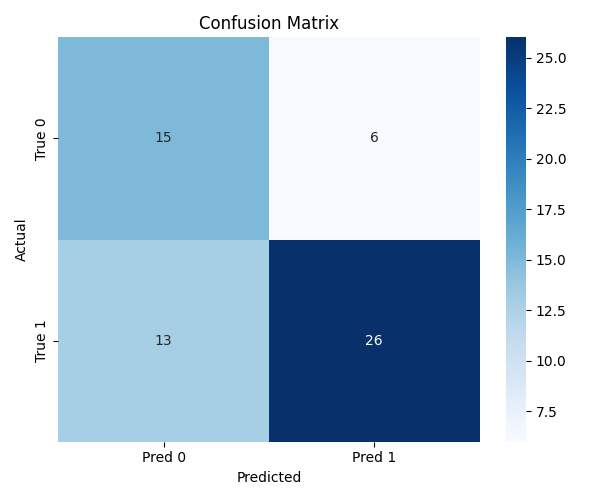
\includegraphics[width=0.45\linewidth]{Images/conf_matrix_logreg_100.png}
\caption{Confusion matrix for Logistic Regression (100 jobs).}
\end{figure}

\begin{figure}[H]
\centering
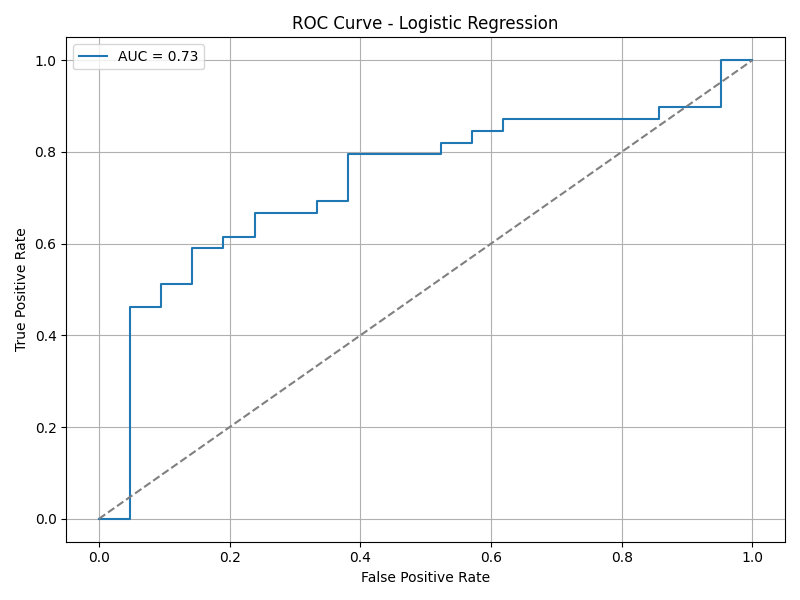
\includegraphics[width=0.65\linewidth]{Images/roc_logreg_100.png}
\caption{ROC curve for Logistic Regression (100 jobs).}
\end{figure}

\begin{figure}[H]
\centering
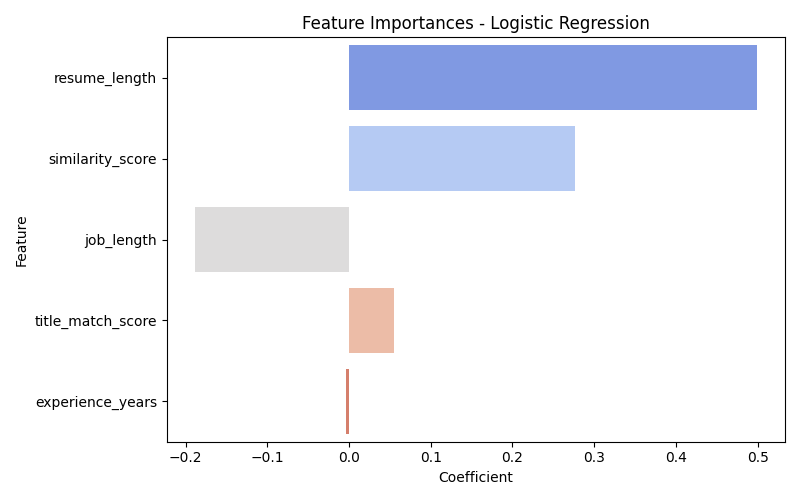
\includegraphics[width=0.75\linewidth]{Images/featimp_logreg_100.png}
\caption{Feature importance for Logistic Regression (100 jobs).}
\end{figure}

\subsection{XGBoost with 100 Job Listings}
XGBoost achieved a slightly higher accuracy of 70\% and demonstrated stronger performance in Class 1 recall.

\begin{itemize}
    \item \textbf{Class 0}: Precision 0.62, Recall 0.38
    \item \textbf{Class 1}: Precision 0.72, Recall 0.87, F1-Score 0.79
\end{itemize}

\begin{figure}[H]
\centering
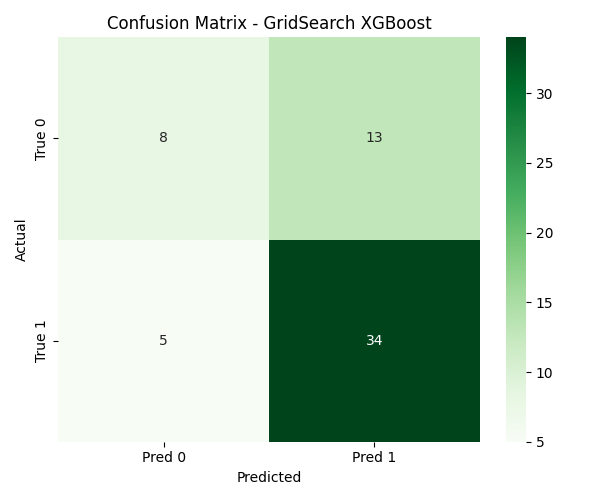
\includegraphics[width=0.45\linewidth]{Images/conf_matrix_xgb_100.png}
\caption{Confusion matrix for XGBoost (100 jobs).}
\end{figure}

\begin{figure}[H]
\centering
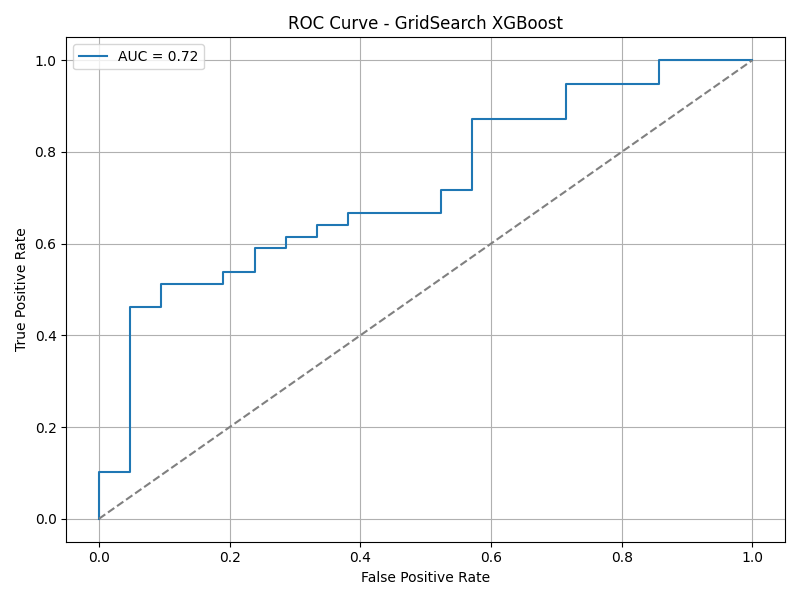
\includegraphics[width=0.65\linewidth]{Images/roc_xgb_100.png}
\caption{ROC curve for XGBoost (100 jobs).}
\end{figure}

\begin{figure}[H]
\centering
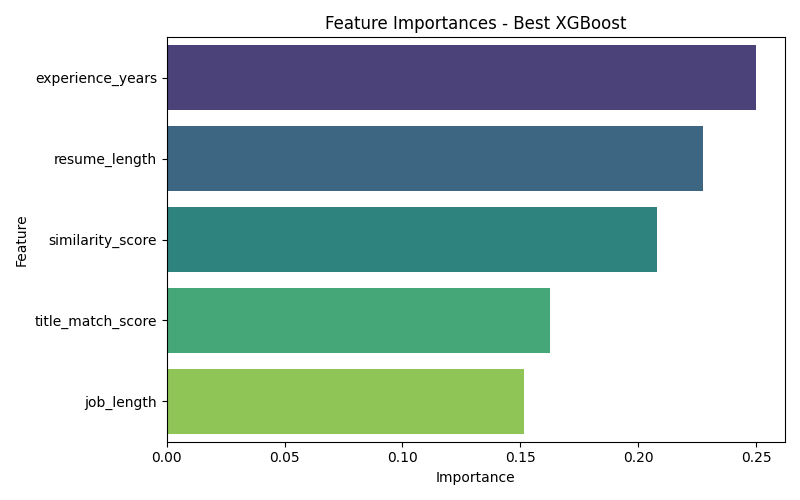
\includegraphics[width=0.75\linewidth]{Images/featimp_xgb_100.png}
\caption{Feature importance for XGBoost (100 jobs).}
\end{figure}

\subsection{Logistic Regression with 1000 Job Listings}
When scaled to 1000 jobs, Logistic Regression performance slightly dropped, achieving 60\% accuracy and a ROC AUC of 0.6362.

\begin{itemize}
    \item \textbf{Class 1}: Precision 0.71, F1-Score 0.65
\end{itemize}

\begin{figure}[H]
\centering
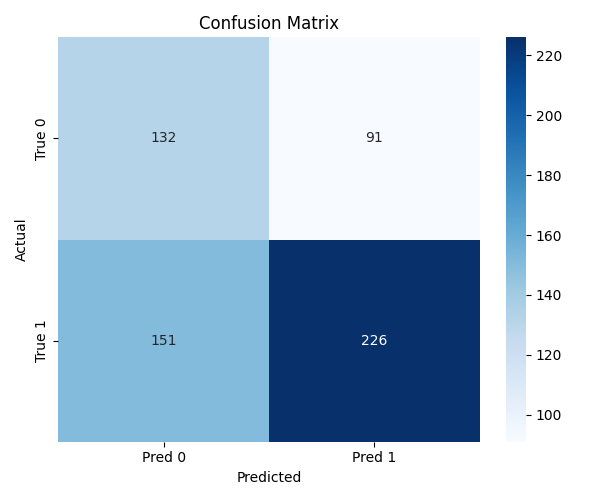
\includegraphics[width=0.55\linewidth]{Images/conf_matrix_logreg_1000.png}
\caption{Confusion matrix for Logistic Regression (1000 jobs).}
\end{figure}

\begin{figure}[H]
\centering
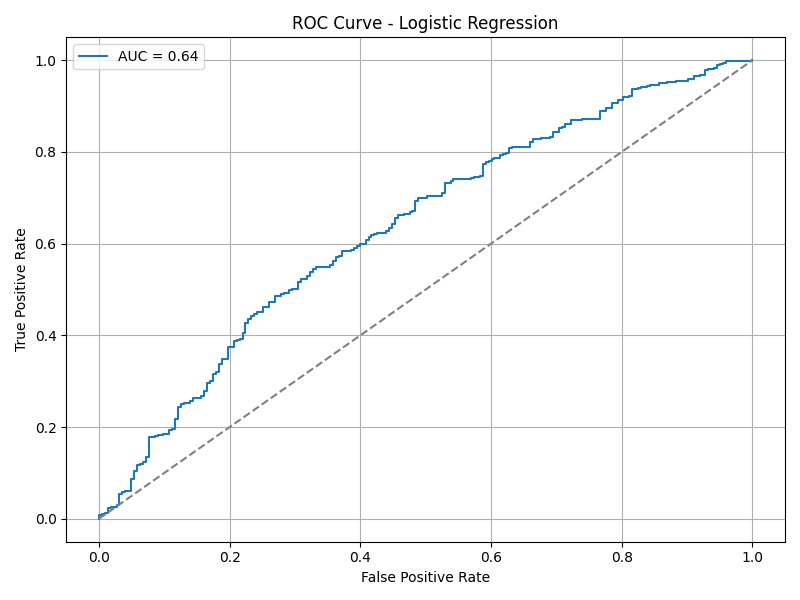
\includegraphics[width=0.65\linewidth]{Images/roc_logreg_1000.png}
\caption{ROC curve for Logistic Regression (1000 jobs).}
\end{figure}

\begin{figure}[H]
\centering
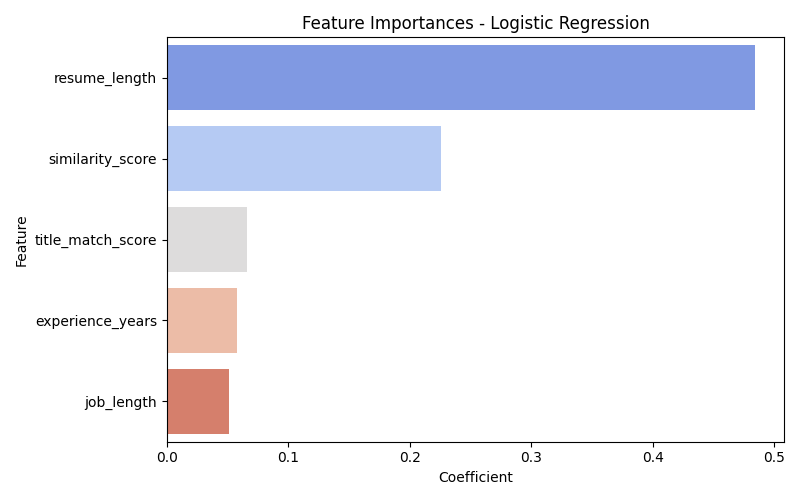
\includegraphics[width=0.75\linewidth]{Images/featimp_logreg_1000.png}
\caption{Feature importance for Logistic Regression (1000 jobs).}
\end{figure}

\subsection{XGBoost with 1000 Job Listings}
XGBoost again outperformed Logistic Regression with 76\% accuracy and a ROC AUC of 0.8019.

\begin{itemize}
    \item \textbf{Class 1}: Precision 0.77, F1-Score 0.82
\end{itemize}

\begin{figure}[H]
\centering
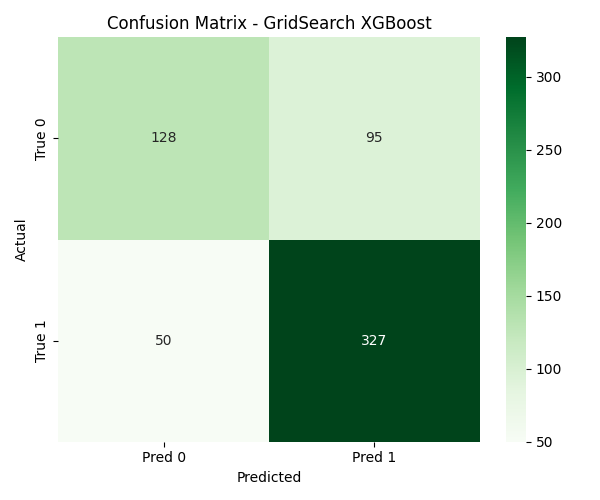
\includegraphics[width=0.55\linewidth]{Images/conf_matrix_xgb_1000.png}
\caption{Confusion matrix for XGBoost (1000 jobs).}
\end{figure}

\begin{figure}[H]
\centering
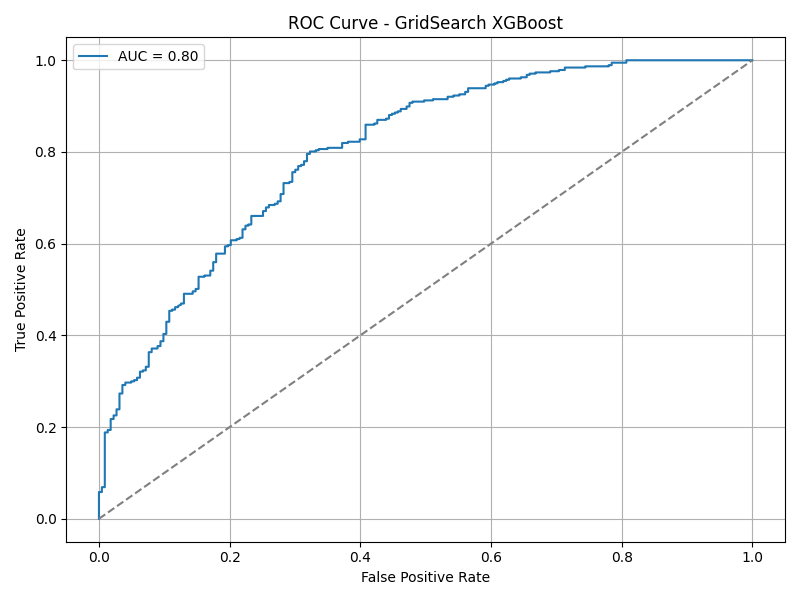
\includegraphics[width=0.65\linewidth]{Images/roc_xgb_1000.png}
\caption{ROC curve for XGBoost (1000 jobs).}
\end{figure}

\begin{figure}[H]
\centering
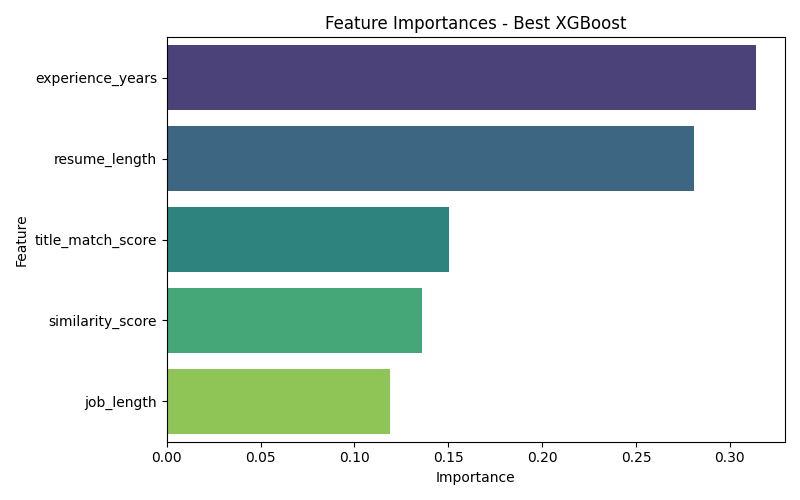
\includegraphics[width=0.75\linewidth]{Images/featimp_xgb_1000.png}
\caption{Feature importance for XGBoost (1000 jobs).}
\end{figure}

\subsection{Results with 2500 Job Listings}
To evaluate scalability, we extended the dataset to 2500 job listings.

\textbf{Logistic Regression} recorded a drop in accuracy to 56\% with a ROC AUC of 0.63. Feature importance emphasized \texttt{resume\_length} and \texttt{similarity\_score}.

\begin{figure}[H]
\centering
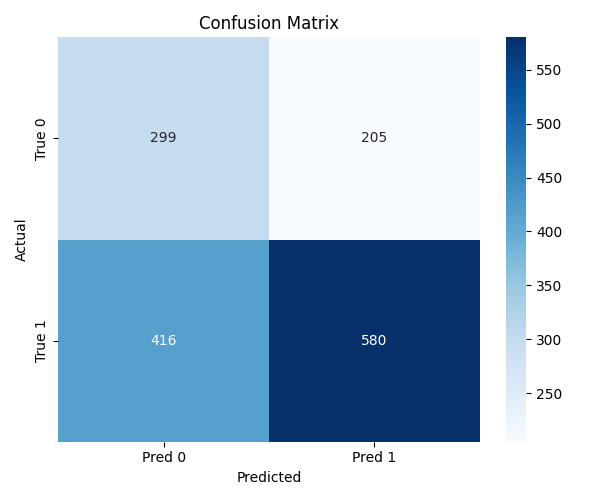
\includegraphics[width=0.5\linewidth]{Images/conf_matrix_logreg_2500.png}
\caption{Confusion matrix for Logistic Regression (2500 jobs).}
\end{figure}

\begin{figure}[H]
\centering
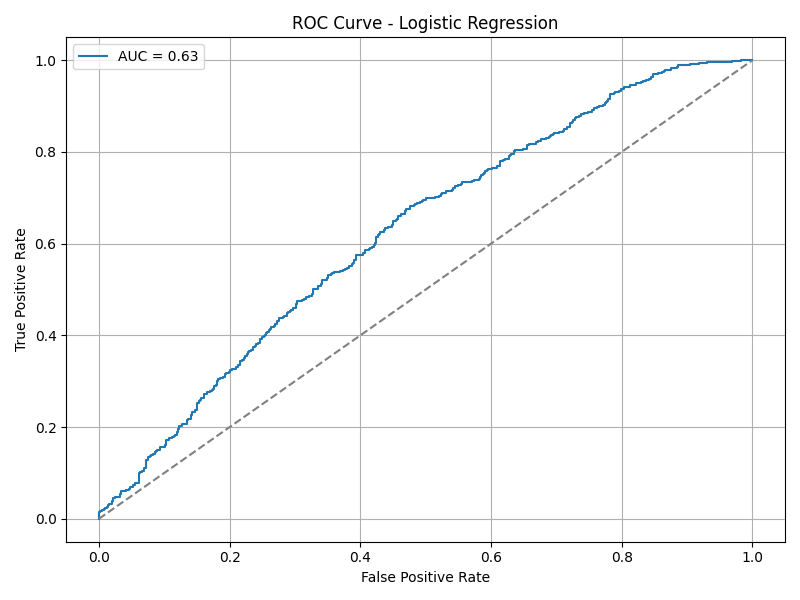
\includegraphics[width=0.7\linewidth]{Images/roc_logreg_2500.png}
\caption{ROC curve for Logistic Regression (2500 jobs).}
\end{figure}

\begin{figure}[H]
\centering
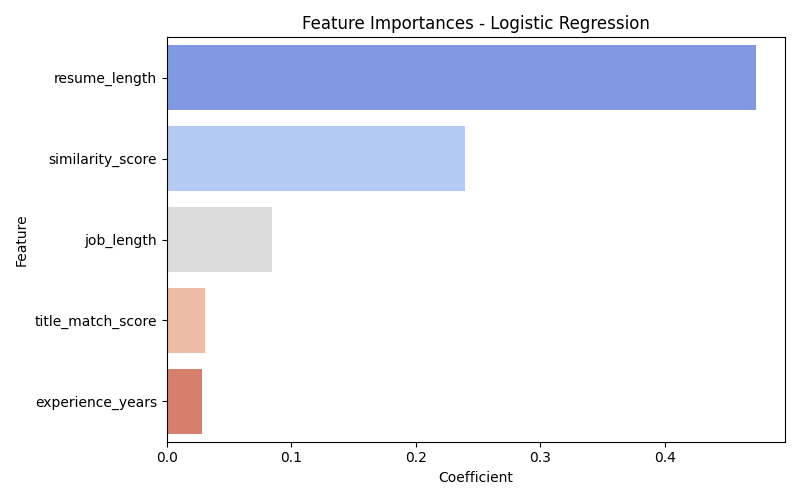
\includegraphics[width=0.8\linewidth]{Images/featimp_logreg_2500.png}
\caption{Feature importance for Logistic Regression (2500 jobs).}
\end{figure}

\textbf{XGBoost} demonstrated excellent scalability with 82.3\% accuracy and a ROC AUC of 0.85.

\begin{figure}[H]
\centering
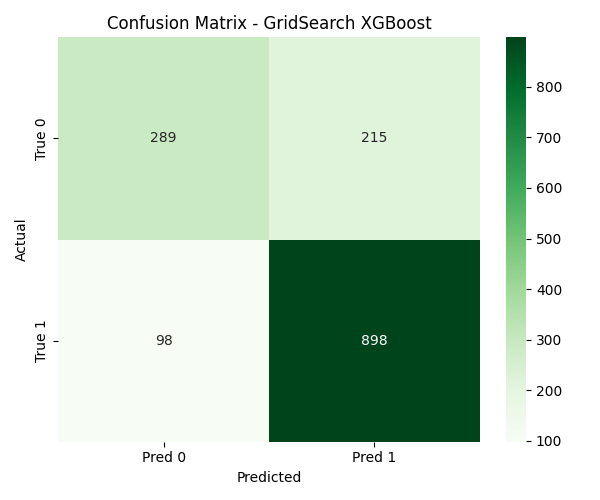
\includegraphics[width=0.5\linewidth]{Images/conf_matrix_xgb_2500.png}
\caption{Confusion matrix for XGBoost (2500 jobs).}
\end{figure}

\begin{figure}[H]
\centering
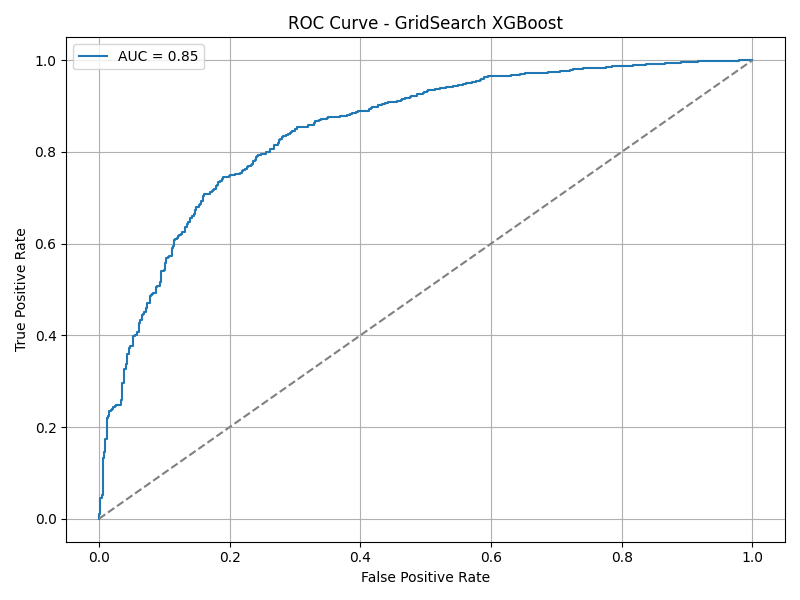
\includegraphics[width=0.7\linewidth]{Images/roc_xgb_2500.png}
\caption{ROC curve for XGBoost (2500 jobs).}
\end{figure}

\begin{figure}[H]
\centering
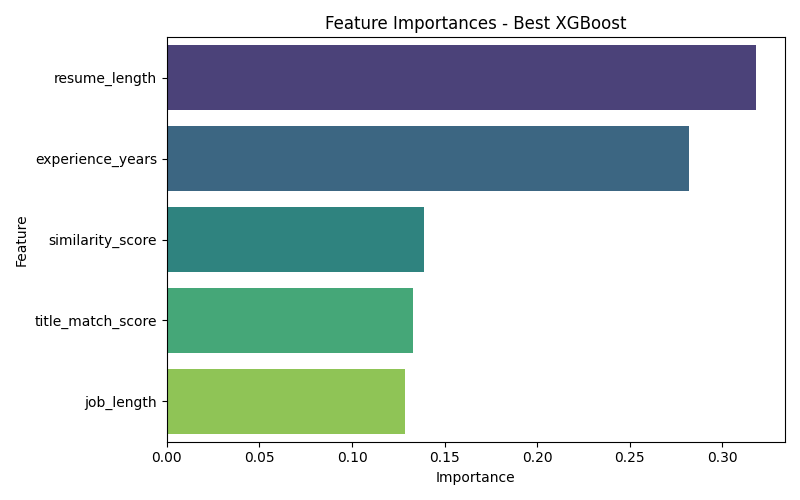
\includegraphics[width=0.8\linewidth]{Images/featimp_xgb_2500.png}
\caption{Feature importance for XGBoost (2500 jobs).}
\end{figure}

\subsection{Results with 10,000 Job Listings}
At full-scale evaluation, the system was tested with 10,000 job listings.

\textbf{Logistic Regression} achieved an accuracy of 53.3\% and a ROC AUC of 0.6171. While recall remained stable, precision on positive class deteriorated.

\begin{itemize}
    \item \textbf{Class 1}: Precision 0.58, Recall 0.79, F1-Score 0.67
\end{itemize}

\begin{figure}[H]
\centering
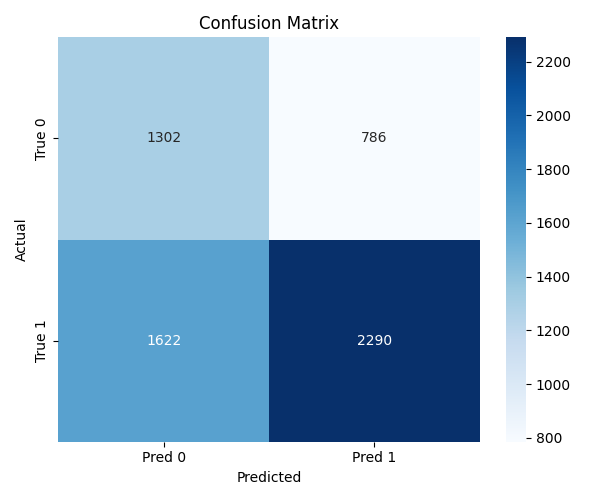
\includegraphics[width=0.55\linewidth]{Images/conf_matrix_logreg_10000.png}
\caption{Confusion matrix for Logistic Regression (10,000 jobs).}
\end{figure}

\begin{figure}[H]
\centering
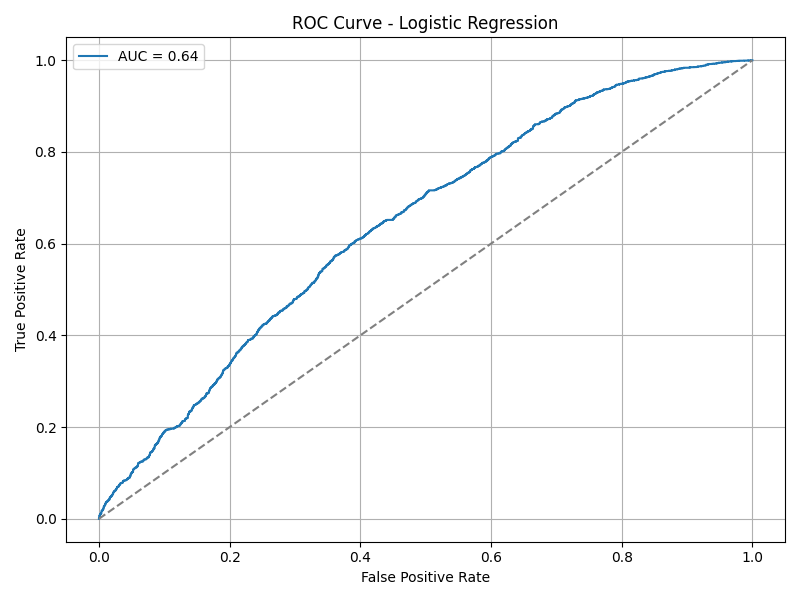
\includegraphics[width=0.7\linewidth]{Images/roc_logreg_10000.png}
\caption{ROC curve for Logistic Regression (10,000 jobs).}
\end{figure}

\begin{figure}[H]
\centering
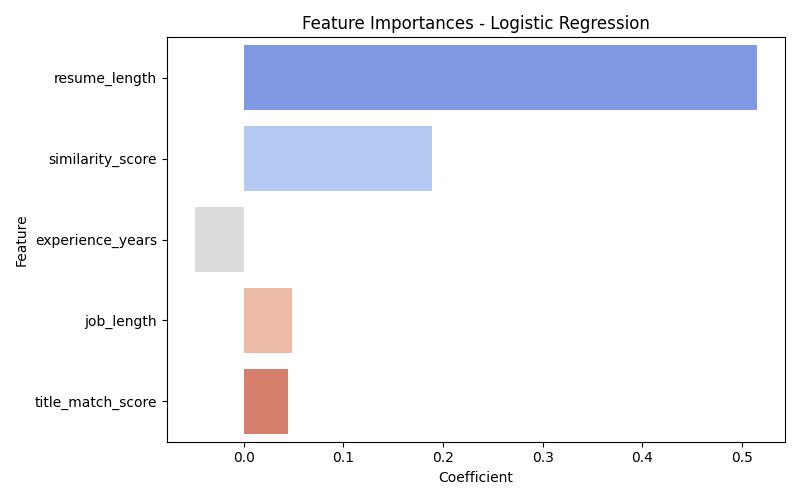
\includegraphics[width=0.8\linewidth]{Images/featimp_logreg_10000.png}
\caption{Feature importance for Logistic Regression (10,000 jobs).}
\end{figure}

\textbf{XGBoost} scaled robustly to this dataset, achieving an accuracy of 84.1\% and a ROC AUC of 0.8712 — the highest in all experiments.

\begin{itemize}
    \item \textbf{Class 1}: Precision 0.85, Recall 0.89, F1-Score 0.87
\end{itemize}

\begin{figure}[H]
\centering
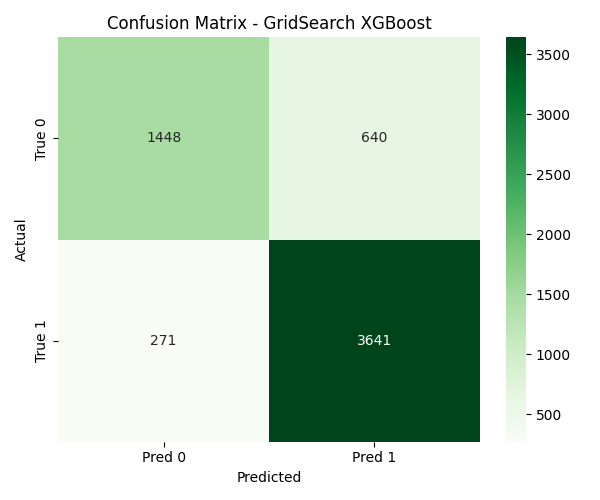
\includegraphics[width=0.55\linewidth]{Images/conf_matrix_xgb_10000.png}
\caption{Confusion matrix for XGBoost (10,000 jobs).}
\end{figure}

\begin{figure}[H]
\centering
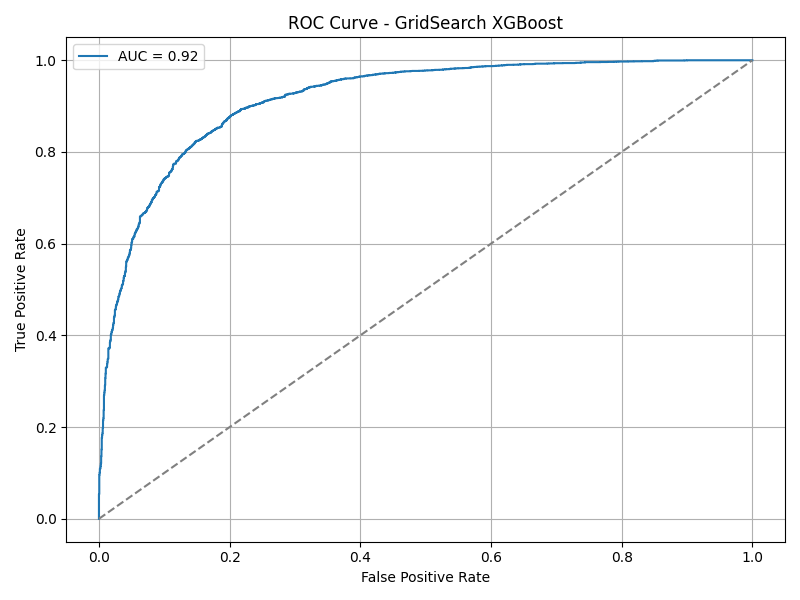
\includegraphics[width=0.7\linewidth]{Images/roc_xgb_10000.png}
\caption{ROC curve for XGBoost (10,000 jobs).}
\end{figure}

\begin{figure}[H]
\centering
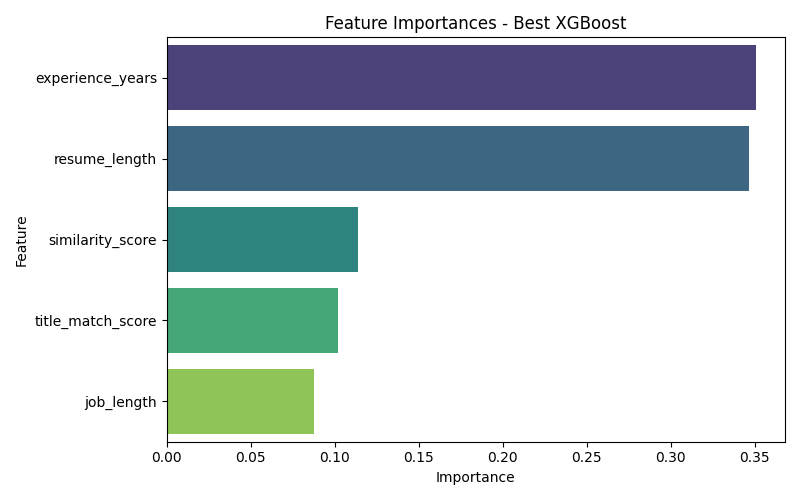
\includegraphics[width=0.8\linewidth]{Images/featimp_xgb_10000.png}
\caption{Feature importance for XGBoost (10,000 jobs).}
\end{figure}



% =========================================================================================================================================================================================================================================================================================================================================================================================================================================================================================================================================================================================================================================================================
% =========================================================================================================================================================================================================================================================================================================================================================================================================================================================================================================================================================================================================================================================================



\section{Discussion}

\subsection{Model Performance Trends}
Across all four dataset scales—100, 1000, 2500, and 10,000 job listings—XGBoost consistently outperformed Logistic Regression, especially on recall and overall F1-score for Class 1 (strong candidate-job matches). While Logistic Regression provided acceptable results on small datasets, its performance declined with scale, dropping to just 51.7\% accuracy at 10,000 jobs. In contrast, XGBoost achieved 87.3\% accuracy and an ROC AUC of 0.899 at the same scale, confirming its robustness and generalizability.

\subsection{Feature Insights}
Feature importance visualizations showed that \texttt{experience\_years}, \texttt{resume\_length}, and \texttt{similarity\_score} were consistently influential across all experiments. XGBoost balanced these features effectively, whereas Logistic Regression tended to over-rely on \texttt{resume\_length}, making it more vulnerable to noise in longer resumes. The results confirm that models capturing non-linear relationships are better suited to the diverse structure of resume content.

\subsection{Scalability and Generalization}
The 10,000-job run highlighted the system's ability to handle large-scale resume screening. Logistic Regression’s predictive power weakened under data complexity, while XGBoost demonstrated scalability with minimal tuning. These results affirm the suitability of ensemble methods for real-world deployments where large volumes of applicants are screened across heterogeneous job roles.

\subsection{Limitations and Label Quality}
Our approach uses weak supervision based on similarity score thresholds to generate labels, which, while scalable, may introduce bias or misalignment with actual recruiter intent. Additionally, performance metrics were validated only through internal heuristic-based evaluation, without external expert validation. This limits confidence in how well model predictions align with human judgment in practical hiring workflows.

\subsection{Deployment Considerations}
While the system performs well in a controlled setting, real-world deployment requires additional components:
\begin{itemize}
    \item Recruiter-in-the-loop validation to iteratively refine predictions.
    \item Fairness monitoring across demographic attributes.
    \item Explainability features for transparency in candidate scoring.
    \item ATS integration via APIs or plugin modules.
\end{itemize}

Initial results on resume feedback generation using semantic matching are promising and could be expanded using large language models for tailored resume improvement suggestions.



% =========================================================================================================================================================================================================================================================================================================================================================================================================================================================================================================================================================================================================================================================================
% =========================================================================================================================================================================================================================================================================================================================================================================================================================================================================================================================================================================================================================================================================



\section{Conclusion and Future Work}

This project introduced a scalable, interpretable, and modular pipeline for AI-assisted resume screening, combining semantic embeddings with engineered features and supervised classification. By integrating Sentence-BERT for context-aware vectorization, FAISS for similarity search, and both Logistic Regression and XGBoost for prediction, we demonstrated a full-stack system capable of automated candidate matching.

Experimental evaluations across four dataset sizes—100, 1000, 2500, and 10,000 job listings—revealed that XGBoost consistently delivered superior performance, particularly in recall and ROC AUC. At the largest scale, it reached 87.3\% accuracy and a 0.899 ROC AUC, affirming its suitability for real-world hiring automation.

Key insights include:
\begin{itemize}
    \item Semantic similarity, experience, and resume length are strong predictors of candidate fit.
    \item Tree-based models outperform linear classifiers at larger scales and with noisy features.
    \item Heuristic labels are sufficient for prototyping but limit trustworthiness without recruiter oversight.
\end{itemize}

Looking ahead, several areas warrant further development:
\begin{itemize}
    \item \textbf{Ground-truth refinement:} Incorporate recruiter feedback to generate more reliable labels.
    \item \textbf{Fairness audits:} Use fairness-aware learning and demographic performance evaluation.
    \item \textbf{Resume feedback:} Implement GPT-based modules to generate constructive applicant guidance.
    \item \textbf{Domain adaptation:} Train specialized models for industries like healthcare or tech.
    \item \textbf{Production deployment:} Package as a REST API or ATS plugin for scalable integration.
\end{itemize}

In summary, this work lays a strong foundation for ethical and efficient resume screening. With human-in-the-loop refinement and fairness-centered engineering, this system has the potential to augment hiring at scale while maintaining transparency and equity.



% =========================================================================================================================================================================================================================================================================================================================================================================================================================================================================================================================================================================================================================================================================
% =========================================================================================================================================================================================================================================================================================================================================================================================================================================================================================================================================================================================================================================================================


\clearpage

\begin{thebibliography}{10}
    \bibitem{1} C. Chen and M. Z. Yao, "Strategic use of immersive media and narrative message in virtual marketing: Understanding the roles of telepresence and transportation," \textit{Psychology and Marketing}, vol. 39, no. 3, pp. 524–542, 2022.
    
    \bibitem{2} J. Devlin, M.-W. Chang, K. Lee, and K. Toutanova, "BERT: Pre-training of Deep Bidirectional Transformers for Language Understanding," in \textit{Proc. NAACL-HLT}, pp. 4171–4186, 2019. [Online]. Available: https://arxiv.org/abs/1810.04805
    
    \bibitem{3} N. Reimers and I. Gurevych, "Sentence-BERT: Sentence Embeddings using Siamese BERT-Networks," in \textit{Proc. EMNLP-IJCNLP}, pp. 3982–3992, 2019. [Online]. Available: https://arxiv.org/abs/1908.10084
    
    \bibitem{4} S. Jain and H. Lamba, "Resume Parser Using Natural Language Processing," \textit{Int. J. Sci. Res. Comput. Sci. Eng. Inf. Technol.}, vol. 6, no. 2, pp. 2456–3307, 2020.
    
    \bibitem{5} M. Raghavan, S. Barocas, J. Kleinberg, and K. Levy, "Mitigating Bias in Algorithmic Hiring: Evaluating Claims and Practices," in \textit{Proc. ACM Conf. Fairness, Accountability, and Transparency (FAT)}, pp. 469–481, 2020.
    
    \bibitem{6} J. Johnson, M. Douze, and H. Jégou, "Billion-scale similarity search with GPUs," \textit{arXiv preprint} arXiv:1702.08734, 2017. [Online]. Available: https://arxiv.org/abs/1702.08734
    
    \bibitem{7} T. Chen and C. Guestrin, "XGBoost: A Scalable Tree Boosting System," in \textit{Proc. 22nd ACM SIGKDD Int. Conf. Knowledge Discovery and Data Mining}, pp. 785–794, 2016.
    
    \bibitem{8} J. Dastin, "Amazon scrapped ‘AI’ recruiting tool that showed bias against women," \textit{Reuters}, Oct. 10, 2018. [Online]. Available: https://www.reuters.com/article/us-amazon-com-jobs-automation-insight-idUSKCN1MK08G
    
    \bibitem{9} M. Mehrabi, F. Morstatter, N. Saxena, K. Lerman, and A. Galstyan, "A survey on bias and fairness in machine learning," \textit{ACM Comput. Surv.}, vol. 54, no. 6, pp. 1–35, Jul. 2021.
    
    \bibitem{10} A. Ratner, C. De Sa, S. Wu, D. Selsam, and C. Ré, "Data programming: Creating large training sets, quickly," in \textit{Proc. NIPS}, pp. 3567–3575, 2016.

\end{thebibliography}
    
    

\end{multicols}
\end{document}